\section{Atividades}

Neste módulo, foram realizadas atividades práticas voltadas à implementação e
ao gerenciamento de certificados digitais em ambientes Windows Server 2022 e
Kali Linux. As tarefas envolveram a criação de uma Autoridade Certificadora
local (CA), a emissão de certificados digitais para clientes da rede e a
aplicação de políticas de inscrição automática de certificados em ambiente de
domínio.

Também foram explorados mecanismos de inspeção e validação de certificados
digitais, tanto em certificados internos emitidos pela autoridade certificadora
local quanto em certificados utilizados por serviços web públicos. Por fim,
foram executados procedimentos de geração de certificados autoassinados no Kali
Linux utilizando a ferramenta OpenSSL, permitindo compreender na prática o
processo completo de criação de chaves privadas, requisições CSR e certificados
X.509.

\newpage

\question[Atividade 9.1]{Criação de Autoridade Certificadora no Windows Server 2022}

\begin{figure}[H]
\centering
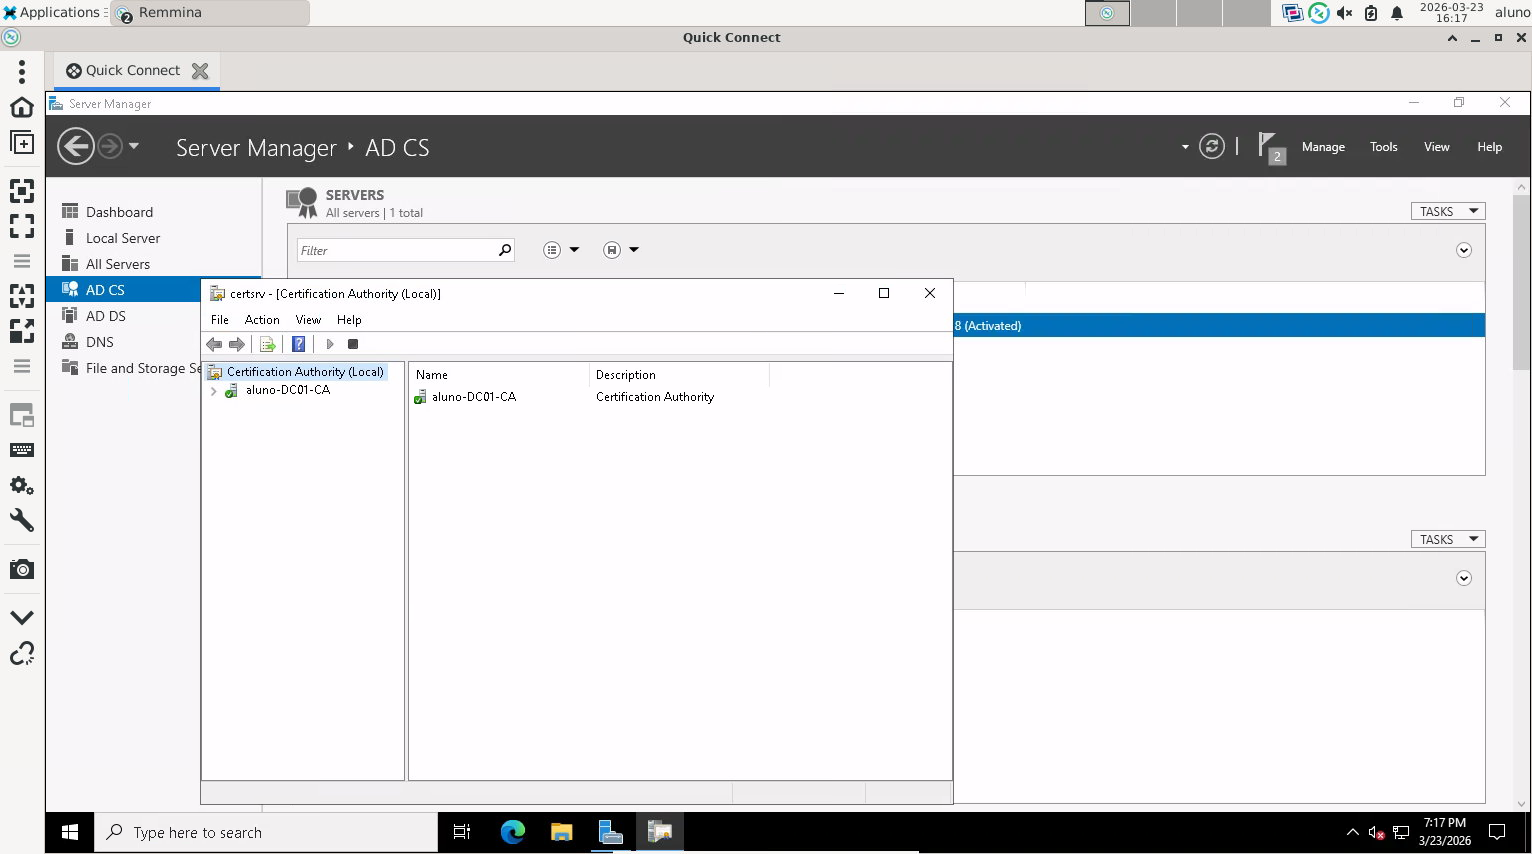
\includegraphics[width=0.99\textwidth]{./fig/fig9.1.png}
\caption{Visualização da autoridade certificadora local aluno-DC01-CA configurada no Windows Server 2022}
\label{fig:fig9.1}
\end{figure}

\newpage

\question[Atividade 9.2]{Emissão de certificados digitais via Group Policy}

\begin{figure}[H]
\centering
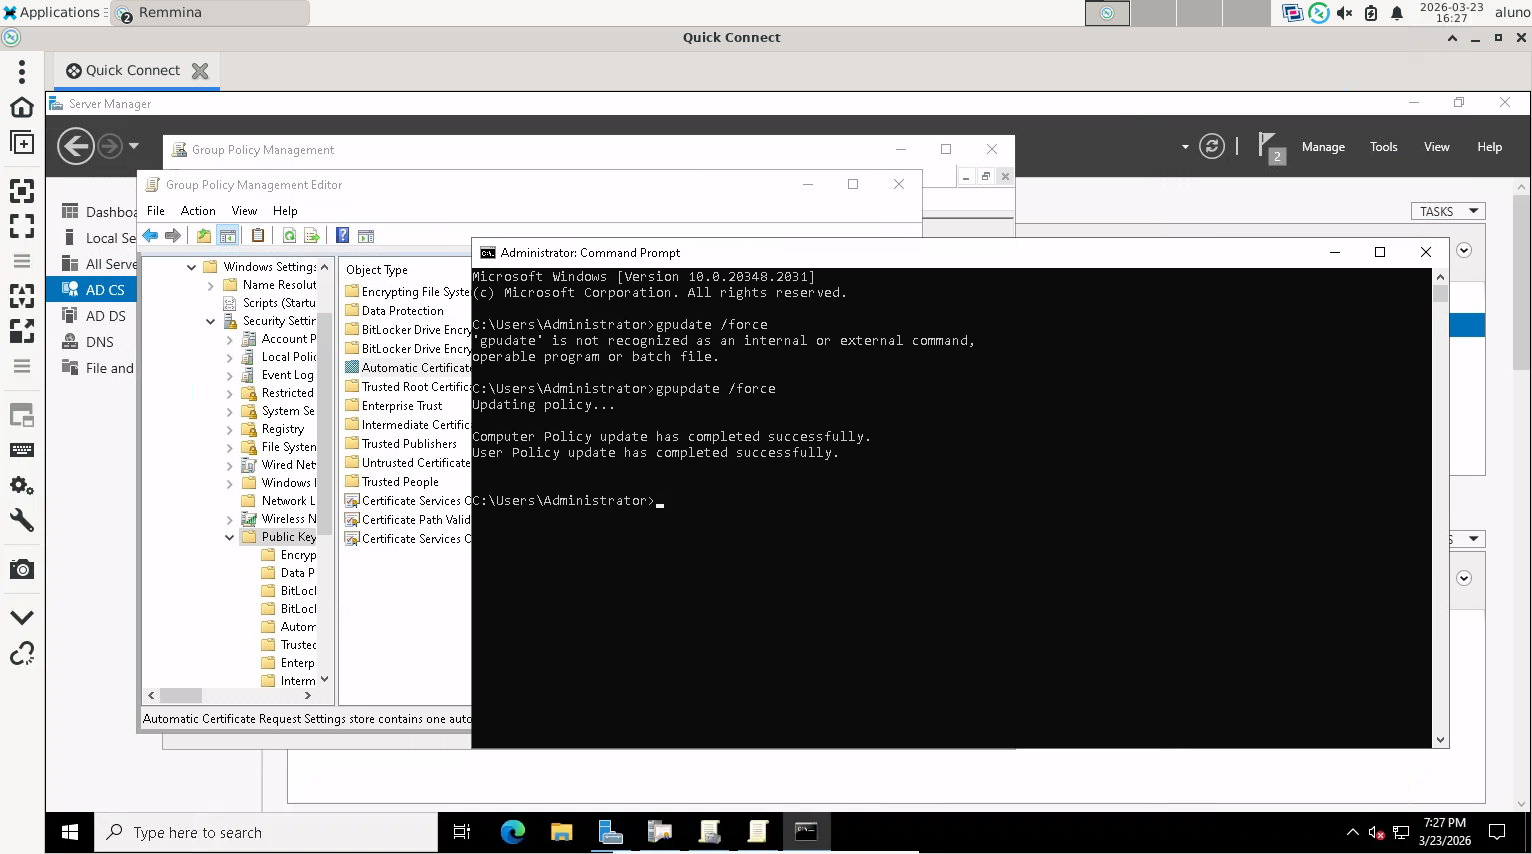
\includegraphics[width=0.99\textwidth]{./fig/fig9.2.png}
\caption{Execução do comando gpupdate /force para aplicar a política de inscrição automática de certificados}
\label{fig:fig9.2}
\end{figure}

\newpage

\question[Atividade 9.3]{Análise de certificado digital no Windows Server 2022}

\begin{figure}[H]
\centering
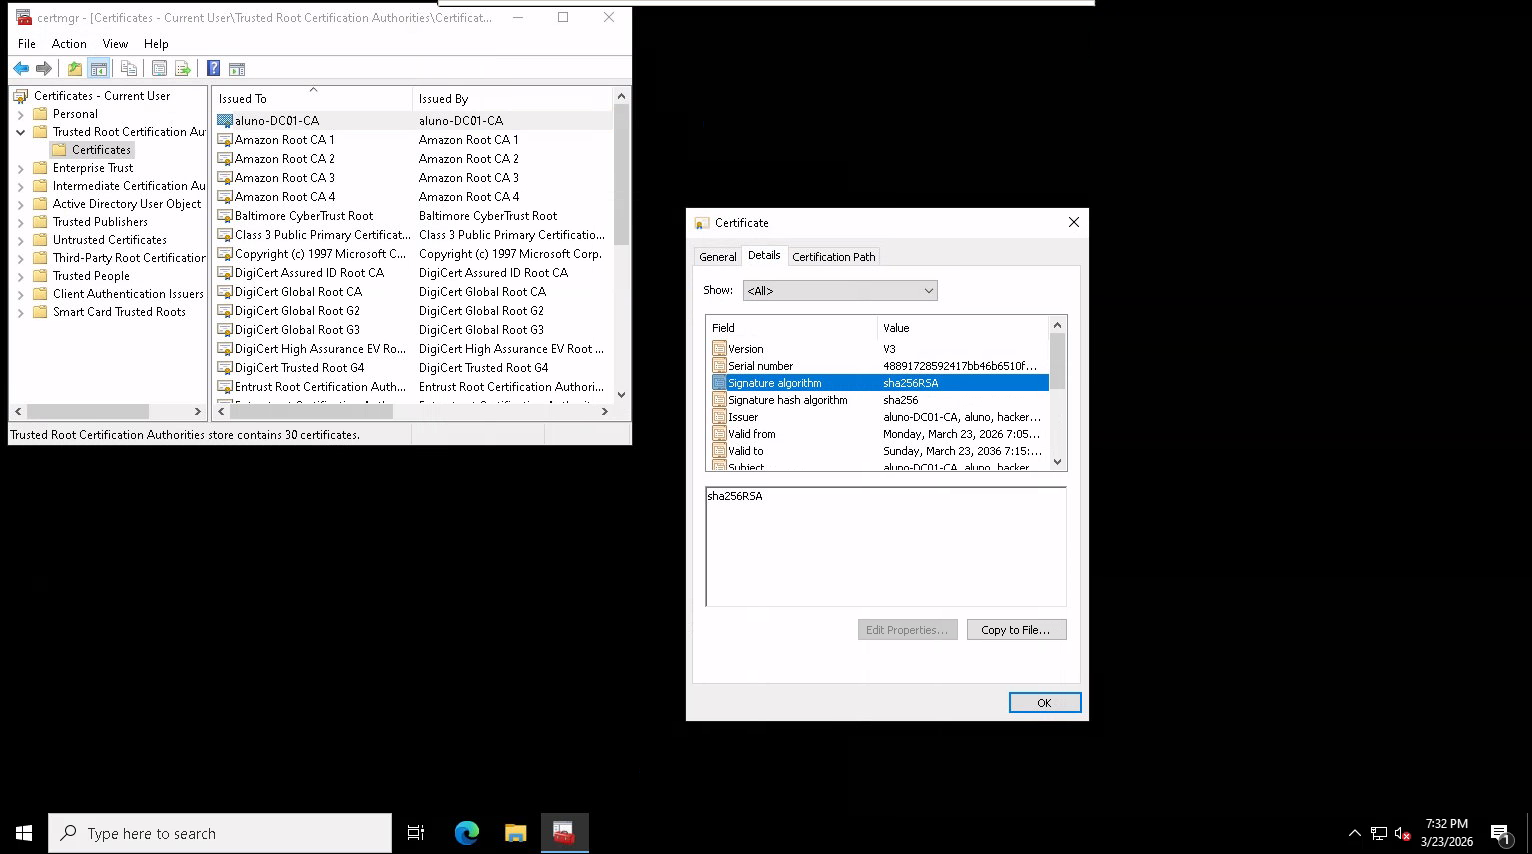
\includegraphics[width=0.99\textwidth]{./fig/fig9.3.png}
\caption{Exibição dos detalhes técnicos do certificado digital emitido pela autoridade certificadora local}
\label{fig:fig9.3}
\end{figure}

\newpage

\question[Atividade 9.4]{Avaliação de certificado web exportado do navegador}

\begin{figure}[H]
\centering
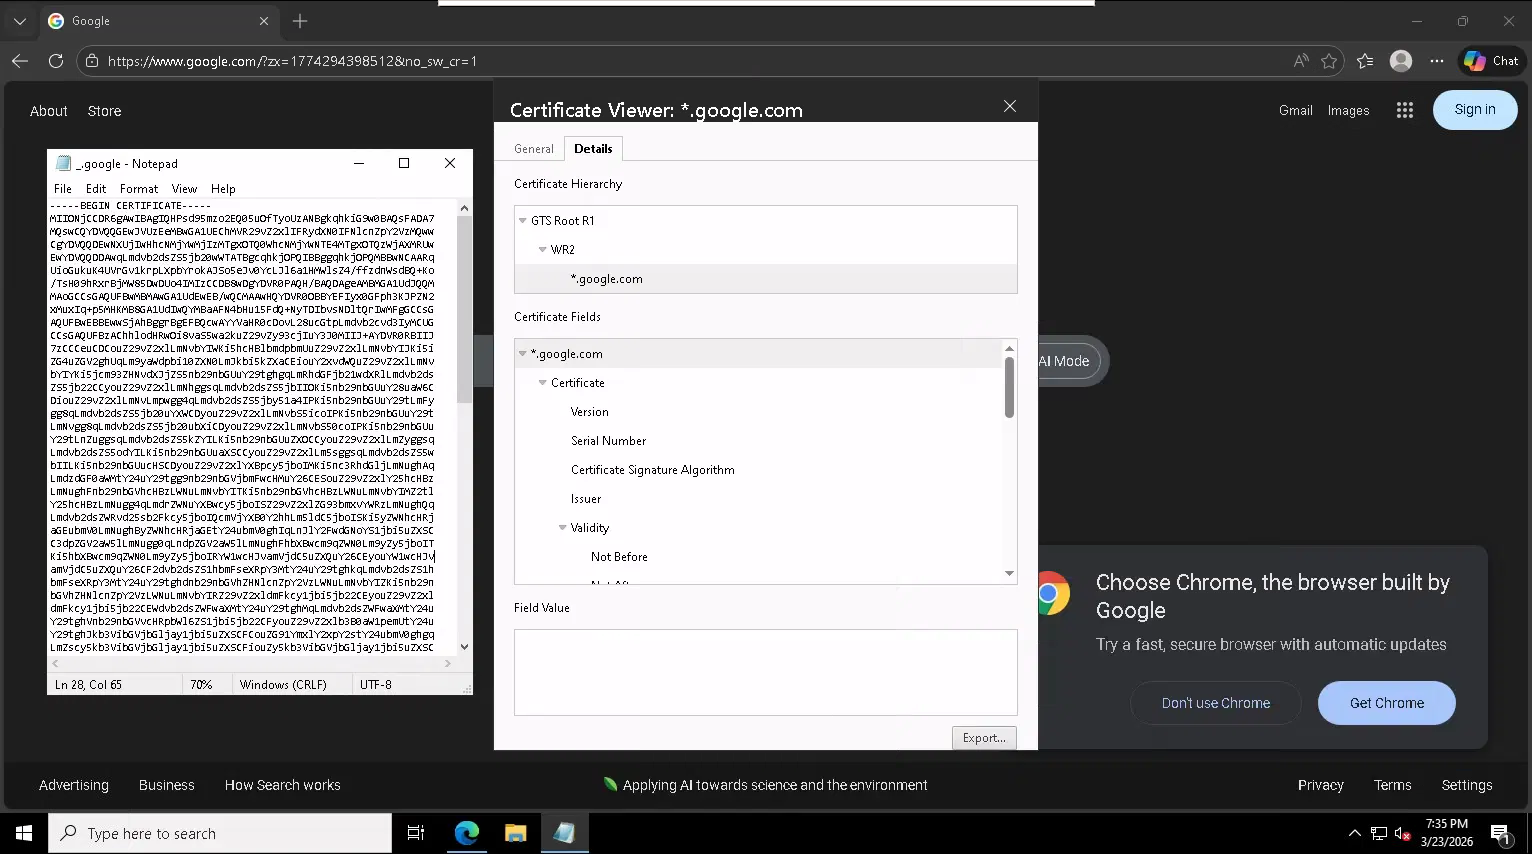
\includegraphics[width=0.99\textwidth]{./fig/fig9.4.png}
\caption{Visualização da estrutura PEM de um certificado digital exportado de um site web}
\label{fig:fig9.4}
\end{figure}

\newpage

\question[Atividade 9.5]{Criação de certificado digital autoassinado no Kali Linux}

\begin{figure}[H]
\centering
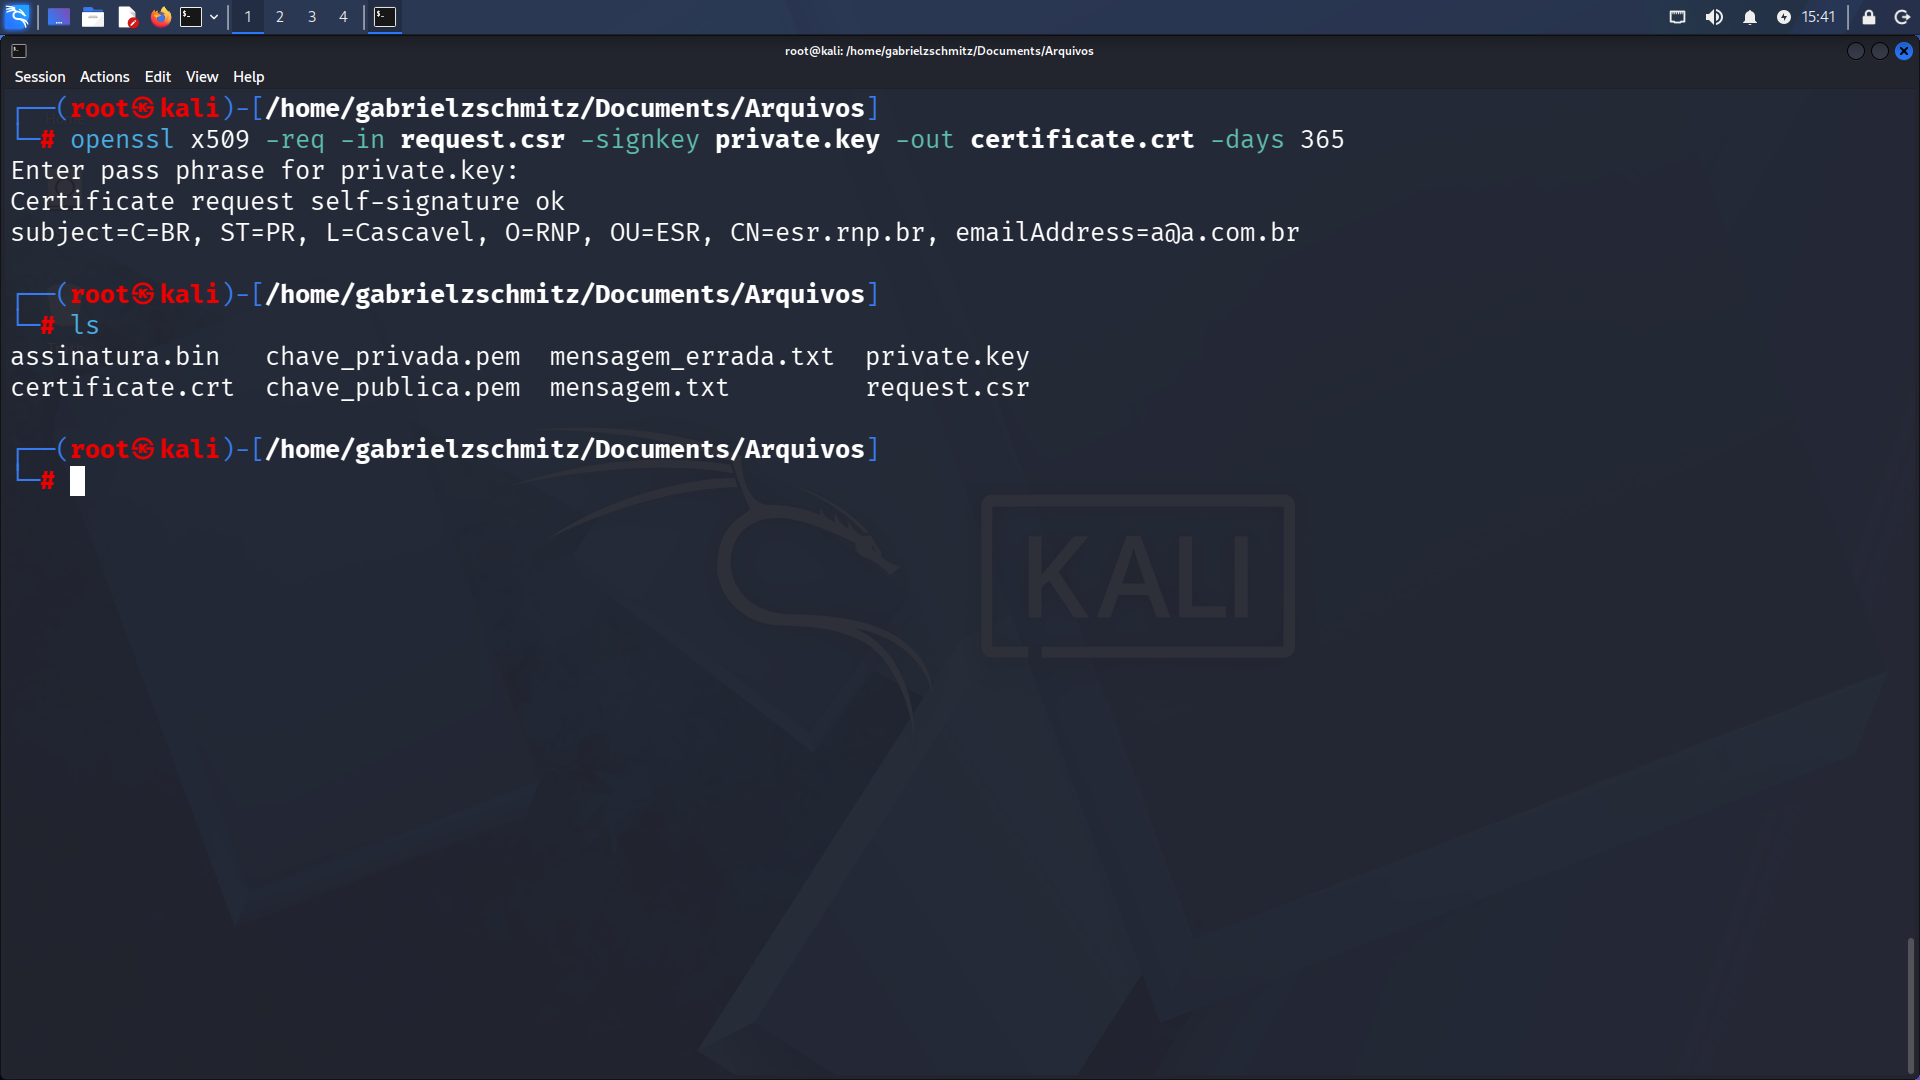
\includegraphics[width=0.99\textwidth]{./fig/fig9.5.png}
\caption{Geração de certificado autoassinado e listagem dos arquivos private.key, request.csr e certificate.crt}
\label{fig:fig9.5}
\end{figure}
